\section{Motivation}
\label{sec:motivation}

This paper develops a DSL for creating GUI animations. This section gives a high-level overview of the problem domain and the expected features of the DSL.

\subsection{Problem Domain}

Graphical user interfaces typically use various concepts to aid users in understanding the current state of the application. One example is to display brief animations whenever the interface changes shape. These type of animations are sometimes called micro-animations.

For example, in Figure~\ref{fig:usecase1} an animation is displayed when the side menu appears on-screen. This menu appears from the right while the background fades out.

\begin{figure}[h]
\centering
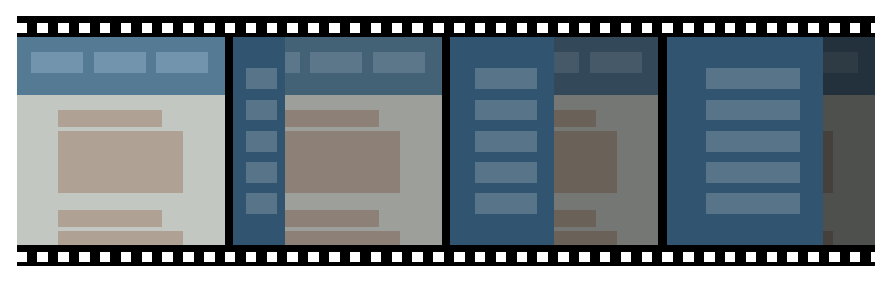
\includegraphics[width=\figscale\textwidth]{pictures/usecase1fig}
\caption{Animation of a side menu appearing while the background fades out.}
\label{fig:usecase1}
\end{figure}

Another example can be seen in Figure~\ref{fig:usecase2}, at the top of the application is a navigation bar. When the user clicks on one of the elements in the bar, an animation is displayed removing the underline from the previously selected element and underlining the newly selected element.

\begin{figure}[h]
\centering
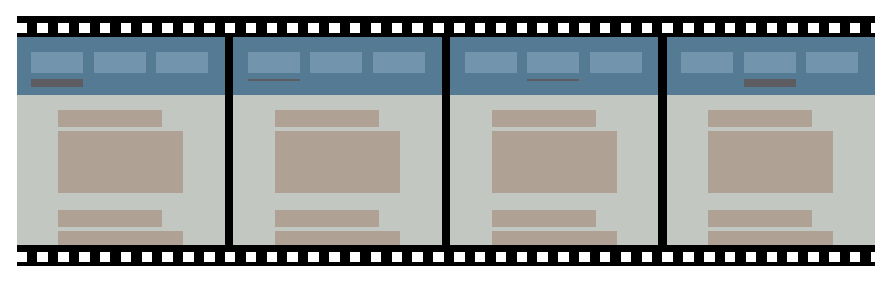
\includegraphics[width=\figscale\textwidth]{pictures/usecase2fig}
\caption{Animation of the underlined element changing in the navigation bar.}
\label{fig:usecase2}
\end{figure}

\subsection{Composing Animations}

The DSL expresses animations by composing smaller parts together. A \emph{basic} animation expresses an elementary unit of animation, which is typically one varying property within the interface. The \emph{composed} animations compose multiple animations into a new animation.

\subsubsection{Basic Animations}

A basic animation changes the value of an element in the UI over a period of time. To specify a basic animation we need three elements: a lens specifying which property in our UI should change, the target value for this property and, lastly, the duration specifying how many seconds the animation should last.

In the menu use case of Figure~\ref{fig:usecase1} there are two properties which need to change during the animation: the \hs{width} of the incoming menu and the alpha property of the box obscuring the application. We express this using the \hs{basic} operation.

First we need to create the animation which makes the side menu appear. We pass three parameters to the \hs{basic} operation: the lens \hs{menu}~\hs{.}~\hs{width} which focuses on the \hs{width} of the incoming menu, the duration \hs{For 0.5} and the target value \hs{To 75}. This results in the animation seen in Figure~\ref{fig:usecase1basic1}.

\begin{spec}
menuSlideIn = basic (menu . width) (For 0.5) (To 75)
\end{spec}

Second we also need to create an animation which fades out the application. Now the lens focuses on the \hs{alpha} value of the obscuring box and sets it to \hs{0.6} over \hs{0.5} seconds. This results in the animation seen in Figure~\ref{fig:usecase1basic2}.

\begin{spec}
appFadeOut = basic (obscuringBox . alpha) (For 0.5) (To 0.6)
\end{spec}

\begin{figure}[h]
\centering

\begin{subfigure}[h]{\textwidth}
\centering
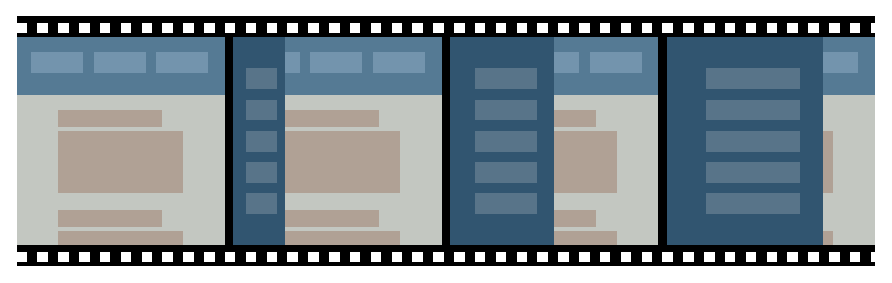
\includegraphics[width=\figscale\textwidth]{pictures/usecase1basic1}
\caption{The \hs{menuSlideIn} animation.}
\label{fig:usecase1basic1}
\end{subfigure}

\begin{subfigure}[h]{\textwidth}
\centering
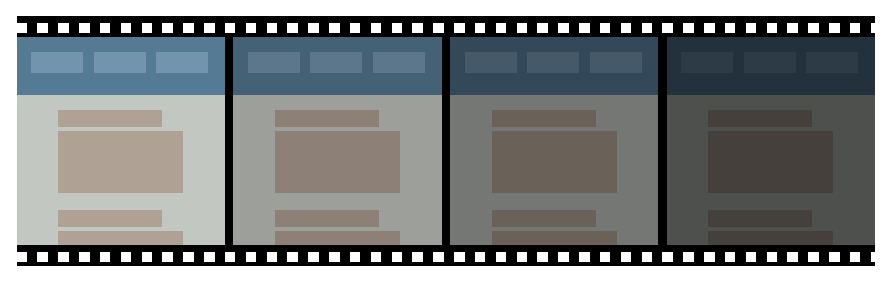
\includegraphics[width=\figscale\textwidth]{pictures/usecase1basic2}
\caption{The \hs{appFadeOut} animation.}
\label{fig:usecase1basic2}
\end{subfigure}

\caption{The \hs{menuAnimation} decomposed into its two elements.}
\label{fig:usecase1basic}
\end{figure}

In the navigation bar use case of Figure~\ref{fig:usecase2} there are again two changing properties: the \hs{height} of the first and second line element. The former is reduced to \hs{0} while the latter is increased to \hs{4}. Again, we create these two animations using the \hs{basic} operation. This results in the animations seen in Figure~\ref{fig:usecase2basic}.

\begin{spec}
decreaseBar1 = basic (navBarLine1 . height) (For 0.25) (To 0)

increaseBar2 = basic (navBarLine2 . height) (For 0.25) (To 4)
\end{spec}

\begin{figure}[h]
\centering

\begin{subfigure}[h]{\textwidth}
\centering
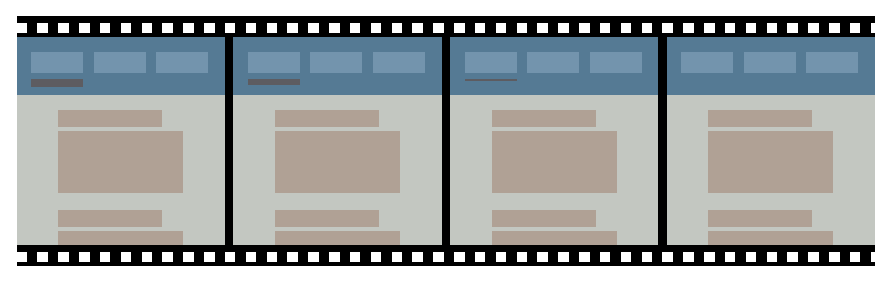
\includegraphics[width=\figscale\textwidth]{pictures/usecase2basic1}
\caption{The \hs{decreaseBar1} animation.}
\label{fig:usecase2basic1}
\end{subfigure}

\begin{subfigure}[h]{\textwidth}
\centering
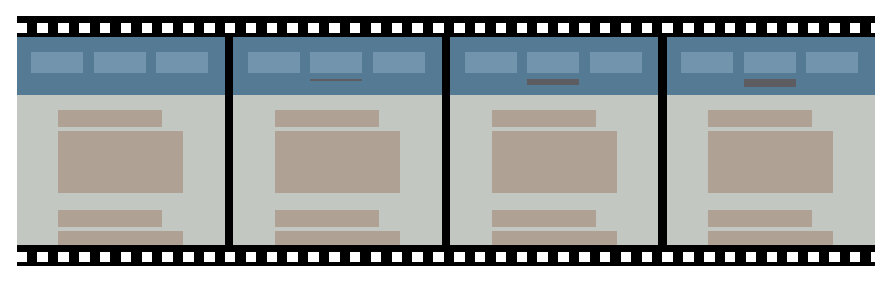
\includegraphics[width=\figscale\textwidth]{pictures/usecase2basic2}
\caption{The \hs{increaseBar2} animation.}
\label{fig:usecase2basic2}
\end{subfigure}

\caption{The \hs{bar2Animation} decomposed into its two elements.}
\label{fig:usecase2basic}
\end{figure}

\paragraph{Lenses} TODO: explain basics of lenses?

\subsubsection{Composed Animations}

A composed animation combines several other animations into one new animation. We can do this either in \emph{sequence} or in \emph{parallel}.

For the menu use case we want to display the animations \hs{menuSlideIn} and \hs{appFadeOut} at the same time. Thus, we create a composed animation using \hs{par},  which results in the animation as seen in Figure~\ref{fig:usecase1}.

\begin{spec}
menuAnimation = menuSlideIn `par` appFadeOut
\end{spec}

For the navigation bar use case we want to display the animations \hs{decreaseBar1} and \hs{increaseBar2} one after the other. To do this we create a composed animation using \hs{seq}, which results in the animation as seen in Figure~\ref{fig:usecase2}.

\begin{spec}
bar2Animation = decreaseBar1 `seq` increaseBar2
\end{spec}

\subsection{Additional Requirements}

In addition to the previous ones, we want to support some additional features: embedding custom operations, embedding custom combinators, and inspecting animations.

\subsubsection{Custom Operations}

The \hs{basic}, \hs{seq}, and \hs{par} operations form the basis for expressing a variety of animations. However, sometimes we need different operations to express our animation. For example, the animation in Figure TODO requires a variety of extra features: randomness, creation and deletion of particles, and setting values within the world. Rather than predicting which operations users will need, the DSL provides the possibility of embedding custom operations.




% Other UI Animation Libraries:
% https://www.codementor.io/hayeskier/7-best-animation-libraries-for-ui-designers-2018-kmg7byy1g
% https://greensock.com/docs/
% https://animejs.com/documentation/#cssSelector

% The DSL also supports embedding of arbitrary operations, by allowing customization of the available operations. For instance, we can add sound effects by creating a \hs{playSound} operation. This operation is then available anywhere an animation.

% In the menu use case for example, we can extend the previous \hs{appFadeOut} animation with a sound effect playing in parallel.

% \begin{spec}
% menuAnimationWithSound = menuAnimation `par` playSound
% \end{spec}

\subsubsection{Inspection}

The DSL is inspectable, meaning that we can derive properties of expressed computations by \emph{inspecting them rather than running them}. For example, we might want to know the duration of \hs{menuAnimation} without actually running it and keeping track of the time. We can do this by using a predefined \hs{duration} function, which calculates the duration by inspecting the animation. This gives a duration of \hs{0.5} seconds, which is indeed the duration of two \hs{0.5} second animations in parallel.

\begin{spec}
menuAnimDuration = duration menuAnimation
-- menuAnimDuration = 0.5 
\end{spec}

Of course, it is not possible to inspect every animation. In the following situation we have a custom operation \hs{getValue} which returns a \hs{Float}. If the result of this value is used as the duration parameter, then we cannot know upfront how long the animation will last. Requesting to calculate the duration of this animation then results in a type error.

\begin{spec}
complicatedAnimation = do
  v <- getValue
  basic lens (For v) (To 10)

compAnimDuration = duration complicatedAnimation
-- type error
\end{spec}

\subsubsection{Custom Combinators}

Similarly to providing custom operations, the DSL also supports custom combinators. For typical DSLs this is not a requirement since working with monadic computations provides the combinators \hs{>>=} and \hs{return} which are suitable for the required use cases. However, since this DSL has the additional requirement of being inspectable, the \hs{>>=} combinator can end up being a liability because it only provide a very limited amount of inspectability. The user is able to use custom combinators, for which they can decide how to inspect them.

Imagine that the user would like to use an \texttt{if-then-else} construction and defines their own combinator \hs{ifThenElse}. Then the user can, similarly to using custom operations, freely mix it with other operations/combinators.

\begin{spec}
rareAnimation =
  ifThenElse
    (fmap (\x -> x == 10) (rng (1, 10))
    specialAnimation
    normalAnimation
\end{spec}

Now it is not possible to inspect the animation to retrieve the exact duration, since \hs{specialAnimation} might have a different duration than \hs{normalAnimation}. Instead, we can retrieve the maximum or minimum duration for the animation.

\begin{spec}
rareAnimMaxDuration = maxDuration rareAnimation
-- rareAnimMaxDuration = 2
\end{spec}

\subsection{Examples}

This section displays some examples of more complicated animations and how they are constructed using the DSL.

TODO: add examples
